% Archivo generado automáticamente con los problemas
\section*{Problems}
Sección: 3_Classical_field_theory
Páginas: 61-64
Contenido:
3.1 Find the generalization of the Euler–Lagrange equations for general Lagrangians,
of the form L [φ, ∂μφ, ∂ν∂μφ, . . .].

3.2 Lorentz currents.
(a) Calculate the conserved currents Kμνα associated with (global) Lorentz
transformations xμ →Λμνxν. Express the currents in terms of the energy-
momentum tensor.
(b) Evaluate the currents for L = 1
2φ

□+ m2
φ. Check that these currents satisfy
∂αKμνα = 0 on the equations of motion.
(c) What is the physical interpretation of the conserved quantities Qi =
!
d3xK0i0
associated with boosts?
(d) Show that dQi
dt = 0 can still be consistent with i ∂Qi
∂t = [Qi, H]. Thus, although
these charges are conserved, they do not provide invariants for the equations of
motion. This is one way to understand why particles have spin, corresponding
to representations of the rotation group, and not additional quantum numbers
associated with boosts.
Problems
43

3.3 Ambiguities in the energy-momentum tensor.
(a) If you add a total derivative to the Lagrangian L →L + ∂μXμ, how does the
energy-momentum tensor change?
(b) Show that the total energy Q =
!
T00 d3x is invariant under such changes.
(c) Show that Tμν ̸= Tνμ is not symmetric for L = −1
4F 2
μν. Can you find an Xμ
so that Tμν is symmetric in this case?

3.4 Write down the next-order diagrams in Eq. (3.85) and their corresponding integral
expressions using Feynman rules. Check that your answer is correct by using the
Green’s function method.

3.5 Spontaneous symmetry breaking is an important subject, to be discussed in depth in
Chapter 28. A simple classical example that demonstrates spontaneous symmetry
breaking is described by the Lagrangian for a scalar with a negative mass term:
L = −1
2φ□φ + 1
2m2φ2 −λ
4!φ4.
(3.86)
(a) How many constants c can you find for which φ(x) = c is a solution to the
equations of motion? Which solution has the lowest energy (the ground state)?
(b) The Lagrangian has a symmetry under φ →−φ. Show that this symmetry
is not respected by the ground state. We say the vacuum expectation value
of φ is c, and write ⟨φ⟩= c. In this vacuum, the Z2 symmetry φ →−φ is
spontaneously broken.
(c) Write φ(x) = c+π(x) and substitute back into the Lagrangian. Show that now
π = 0 is a solution to the equations of motion. How does π transform under
the Z2 symmetry φ →−φ? Show that this is a symmetry of π’s Lagrangian.

3.6 Yukawa potential.
(a) Calculate the equations of motion for a massive vector Aμ from the Lagrangian
L = −1
4F 2
μν + 1
2m2A2
μ −AμJμ,
(3.87)
where Fμν = ∂μAν −∂νAμ. Assuming ∂μJμ = 0, use the equations to find a
constraint on Aμ.
(b) For Jμ the current of a point charge, show that the equation of motion for A0
reduces to
A0(r) =
e
4π2ir
 ∞
−∞
k dk
k2 + m2 eikr.
(3.88)
(c) Evaluate this integral with contour integration to get an explicit form for A0(r).
(d) Show that as m →0 you reproduce the Coulomb potential.
(e) In 1935 Yukawa speculated that this potential might explain what holds protons
together in the nucleus. What qualitative features does this Yukawa potential
have, compared to a Coulomb potential, that make it a good candidate for the
force between protons? What value for m might be appropriate (in MeV)?
(f) Plug the constraint on Aμ that you found in part (a) back into the Lagrangian,
simplify, then rederive the equations of motion. Can you still find the con-
straint? What is acting as a Lagrange multiplier in Eq. (3.87)?
44
Classical field theory

3.7 Nonlinear gravity as a classical field theory. In this problem, you will calculate the
perihelion shift of Mercury simply by dimensional analysis.
(a) The interactions in gravity have
L = M 2
Pl
−1
2hμν□hμν + (∂αhμν)(∂βhμα)hνβ + · · ·
−hμνTμν, (3.89)
where MPl =
1
√GN is the Planck scale. Rescaling h, and dropping indices and
numbers of order 1, this simplifies to
L = −1
2h□h + (MPl)ah2□h −(MPl)bhT.
(3.90)
What are a and b (i.e. what are the dimensions of these terms)?
(b) The equations of motion following from this Lagrangian are (roughly)
□h = (MPl)a□(h2) −(MPl)bT.
(3.91)
For a point source T = mδ(3)(x), solve Eq. (3.91) for h to second order in the
source T (or equivalently to third order in M −1
Pl ). You may use the Coulomb
solution we already derived.
(c) To first order, h is just the Newtonian potential. This causes Mercury to
orbit. What is Mercury’s orbital frequency, ω = 2π
T ? How does it depend on
mMercury, mSun, MPl and the distance R between Mercury and the Sun?
(d) To second order, there is a correction that causes a small shift Mercury’s orbit.
Estimate the order of magnitude of the correction to ω in arcseconds/century
using your second-order solution.
(e) Estimate how big the effect is of other planets on Mercury’s orbital fre-
quency. (Dimensional analysis will do – just get the right powers of masses
and distances.)
(f) Do you think the shifts from either the second-order correction or from the
other planets should be observable for Mercury? What about for Venus?
(g) If you derive Eq. (3.91) from Eq. (3.90), what additional terms do you get?
Why is it OK to use Eq. (3.91) without these terms?

3.8 How does the blackbody paradox argument show that the electromagnetic field
cannot be classical while electrons and atoms are quantum mechanical? Should
the same arguments apply to treating gravity classically and electrons quantum
mechanically?

3.9 Photon polarizations (this problem follows the approach in [Feynman et al., 1996]).
(a) Starting with L = −1
4F 2
μν+JμAμ, substitute in Aμ’s equations of motion. This
is called integrating out Aμ. In momentum space, you should get something
like Jμ 1
k2 Jμ.
(b) Choose kμ = (ω, κ, 0, 0). Use current conservation (∂μJμ = 0) to formally
solve for J1 in terms of J0, ω and κ in this coordinate system.
(c) Rewrite the interaction Jμ 1
k2 Jμ in terms of J0, J2, J3, ω and κ.
(d) In what way is a term without time derivatives instantaneous (non-causal)?
How many causally propagating degrees of freedom are there?

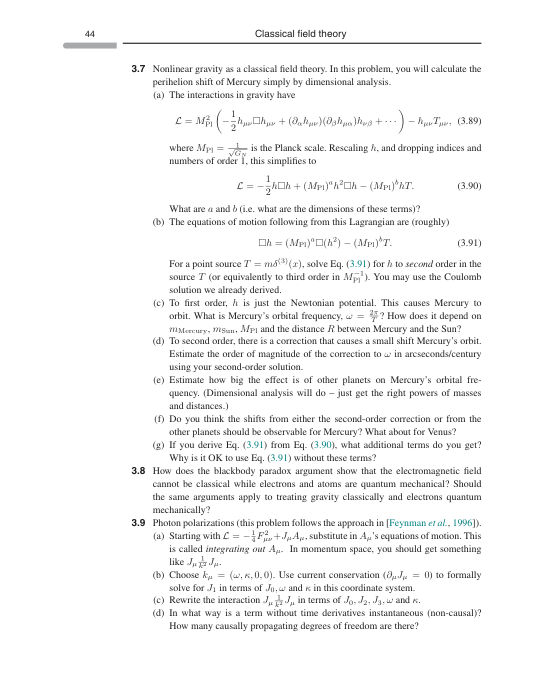
\includegraphics{./figs/3_Classical_field_theory_page_64.png}

---

